% !TeX root = ../main.tex

\chapter{Single resource systems}
\label{ch:single-resource}
This chapter studies uplink NOMA with single resource system, where PD-NOMA with soft SIC and GDMA ~\cite{hsu2019gain} are discussed. 
We assume that the channel state information (CSI) is perfectly known at the receiver. The performance of these two detection schemes is evaluated in terms of bit error rate (BER) under different large scale fading coefficients.
\begin{comment}
Last, we clarify the performance gap between GDMA detection and soft SIC detection under different large scale fading coefficients.
\end{comment}

\begin{comment}
Last, we compare the bit error rate(BER) performance of this two detectors.
\end{comment}


\section{Single resource system model}
Consider an uplink system where perfect timing synchronization is assumed. $U$ users transmit simultaneously over one shared resource, which may be a frequency band, time slot, or spreading signature. The received signal at the BS is
\begin{equation}
    \label{eq:single_resource_system_model}
    y = \sum_{k=1}^{U} \sqrt{P_k \beta_k} h_k x_k + n,
\end{equation}
where $P_k$ is the transmit power of user $k$, $\beta_k$ is the large-scale fading coefficient of user $k$, $h_k$ is the small-scale Rayleigh flat-fading coefficient of user $k$, $x_k$ is transmission symbol of user $k$ and $n \sim \mathcal{CN}(0,N_0)$ is complex AWGN. 
Equivalently, the noise variance per dimension is $\sigma^2=N_0/2$. 
In this work, for simplicity, $P_k=1$ is assumed unless otherwise stated.

\section{Detection principle for PD NOMA : soft SIC}
\label{sec:Detection principle for PD NOMA : soft SIC}
In PD-NOMA, users are mainly separated by their received-power difference. The instantaneous received-power metric of user $k$ can be written as
\begin{equation}
    \rho_k = P_k\beta_k |h_k|^2 \triangleq |g_k|^2.
\end{equation}
The SIC detection order is denoted by
\begin{equation}
    \pi=\{\pi(1),\pi(2),\ldots,\pi(U)\},
\end{equation}
where $\pi(i)$ is the user detected at stage $i$. For received power-based ordering, this order is usually determined such that
    $\rho_{\pi(1)} \geq \rho_{\pi(2)} \geq \cdots \geq \rho_{\pi(U)}$.
The user indices are then relabeled according to this order.
For simplicity, we assume the user indices in \eqref{eq:single_resource_system_model} have been renumbered, so that the $i^{th}$ SIC stage detects the LLR of user $i$, denoted $L_{x_i}$.

At the first SIC stage, the LLR of $x_1$, $L_{x_1}$, is obtained by regarding signals from other users as approximately Gaussian in \eqref{eq:single_resource_system_model} and the soft estimate is denoted as $\hat{s}_{1}$.
At the $(i+1)^{th}$ SIC stage, the LLR of $x_{i+1}$, $L_{x_{i+1}}$, is obtained by a residual signal $y_{(i+1)}$ which is obtained by subtracting the contribution of the soft estimate $\hat{s}_{i}$ in the $i^{th}$ stage and regarding signals from other users as Gaussian. Therefore, 
\begin{equation}
    y_{(1)} = y,
\end{equation}
\begin{equation}
 \label{eq:subtract}
    y_{(i+1)}
    =
    y_{(i)}
    -
    g_{i}\hat{s}_{i}.
\end{equation}
For BPSK modulation, the log likelihood ratio (LLR) of user $i$ can be simplified as
\begin{equation}
    \label{eq:LLR}
    L_{x_i}
    =
    \log
    \frac{
    p(y_{(i)}|x_{\pi(i)}=+1)
    }{
    p(y_{(i)}|x_{\pi(i)}=-1)
    }
    =
    \frac{
    4\Re\{
    g_{i}^* y_{(i)}\}
    }{
    \sigma_{\mathrm{eff},(i)}^{2}
    }.
\end{equation}
The soft estimate of the detected symbol given $y_{(i)}$ is expressed ~\cite{shapiro2005soft} by
\begin{equation}
    \label{eq:soft calculation}
    \hat{s}_{i}
    =
    \mathbb{E}\left[x_{i}|L_{x_i}\right]
    =
    \tanh\left(\frac{L_{x_i} }{2}\right).
\end{equation}
and the conditional variance is obtained ~\cite{shapiro2005soft} as
\begin{equation}
    \label{eq:soft variance}
    \sigma^2_{\hat{s}_i}
    =
    \mathbb{E}\left[x^2_i|L_{x_i}\right]
    =
    1-\tanh^2 \left(\frac{L_{x_i}}{2}\right).
\end{equation}
Therefore, the effective noise variance is
\begin{equation}
    \sigma_{\mathrm{eff},{(i)}}^2
    =
    2\sigma^2
    +
    \sum_{j=i+1}^{U}
    |g_{j}|^2
    + 
    \sum_{j=1}^{i-1}
    \sigma^2_{\hat{s}_{j}}.
\end{equation}
The first term is the noise variance, the second term is the interference from undetected users, and the third term is the uncertain residual interference from previously detected users.
This procedure is repeated until all users are detected.

\section{Detection principle for GDMA}
\label{sec:Detection principle for GDMA}

In GDMA, users are distinguished by their distinct channel gains. Unlike PD-NOMA, which relies mainly on received-power differences, GDMA uses both the magnitude and phase of $g_k$.

\begin{table}[htbp]
        \centering
        \caption{Mapping rules for superimposed signal in the case of $M = 1$ and $U = 2$}
        \renewcommand{\arraystretch}{1.5} % 增�?每�??��?高度
        \setlength{\tabcolsep}{10pt}      % 增�?欄�?左右?��?
        \resizebox{1.15\width}{!}{
      \begin{tabular}{|c|c|c|c|c|c|}
        \hline
        $l$  & $x_1$ & $x_2$ & $s_l$ \\ \hline
        0 & 1 & 1 & $\sqrt{\beta_1}h_1 + \sqrt{\beta_2}h_2$ \\ \hline
        1 & 1 & -1 & $\sqrt{\beta_1}h_1 - \sqrt{\beta_2}h_2$ \\ \hline
        2 & -1 & 1 & $-\sqrt{\beta_1}h_1 + \sqrt{\beta_2}h_2$ \\ \hline
        3 & -1 & -1 & $-\sqrt{\beta_1}h_1 - \sqrt{\beta_2}h_2$ \\ \hline
      \end{tabular}
      }
      
      \label{table:superimposed-bpsk-u2}
\end{table}

At the receiver, the superimposed signal is first used to calculate the $a$ $posteriori$ probabilities (APPs) of all possible combinations of multiuser symbols, and then the LLR of each user is then obtained accordingly ~\cite{hsu2019gain}. There are $2^{MU}$ possible superimposed signal levels, denoted by the set
\begin{equation}
    \mathcal{S}
    =
    \{s_0,s_1,\ldots,s_{2^{MU}-1}\},
\end{equation}
where $M$ is the number of coded bits per modulation symbol for each user and $s_l\in\mathcal{S}$ contributes to the signal part in \eqref{eq:single_resource_system_model}. 
Take BPSK modulation ($M=1$) as an example, the superimposed signal 
\begin{equation}
  \begin{split}
    s_l &= (-1)^{l_2[1]} \cdot \sqrt{\beta_1}h_1 + (-1)^{l_2[2]} \cdot \sqrt{\beta_2}h_2 + \cdots + (-1)^{l_2[U]} \cdot \sqrt{\beta_U}h_U \\
    &= \sum_{k=1}^{U} (-1)^{l_2[k]} \cdot \sqrt{\beta_k}h_k, \quad l=0,1,\ldots,2^U-1,
  \end{split}
\end{equation}
where $l_2[k]$ denotes the transmission bit of user $k$ in the binary representation. 

In detail: 
\begin{equation}
  \begin{aligned}
    l=0 &\rightarrow (l_2[1], l_2[2], \ldots, l_2[U]) = (0, 0, \ldots, 0) \\
    l=1 &\rightarrow (l_2[1], l_2[2], \ldots, l_2[U]) = (0, 0, \ldots, 1) \\
    &\vdots \\
    l=2^U-1 &\rightarrow (l_2[1], l_2[2], \ldots, l_2[U]) = (1, 1, \ldots, 1).
  \end{aligned}
\end{equation}
The superimposed signal levels $s_l$ for the case $U=2$ are listed in Table~\ref{table:superimposed-bpsk-u2}, where $l \in \{0,1,2,3\}$.

The receiver computes the $a$ $posteriori$ probabilities (APPs) of each possible superimposed signal $s_l\in\mathcal{S}$ by
\begin{equation}
    P(s_l|y) = P(y|s_l) \cdot \frac{P(s=s_l)}{P(y)}. 
\end{equation}
Assuming the signals in $\mathcal{S}$ are equally probable, the APPs can be formulated as
\begin{equation}
    P(s_l|y)  \propto\exp\left(-\frac{|y-s_l|^2}{2\sigma^2}\right).
\end{equation}
The log-likelihood ratio (LLR) of user $k$ is then calculated by
\begin{equation}
    L_{x_k} =
    \log
    \frac{
    \sum\limits_{ {x_k}=+1}
    \exp\left(-\frac{|y-s_l|^2}{2\sigma^2}\right)
    }{
    \sum\limits_{ {x_k}=-1}
    \exp\left(-\frac{|y-s_l|^2}{2\sigma^2}\right)
    }.
\end{equation}

\section{Simulations of PD NOMA with soft SIC and GDMA}
The single-resource simulations use BPSK modulation for each user over independent Rayleigh flat-fading channels. 
Figure~\ref{fig:single-resource-ber-1-1}, 
~\ref{fig:single-resource-ber-1-0-1} and 
~\ref{fig:single-resource-ber-1-0-01} show the BER performance of two users with different large-scale fading coefficients $(\beta_1, \beta_2)$.
As the large-scale fading gap becomes larger, the soft SIC detection converges toward the performance of the GDMA detection, indicating that the received-power disparity provides a clearer detection order and reduces the ambiguity of early cancellation stages. However, it comes at the severe cost of user fairness ~\cite{ding2015impact}.

Figure~\ref{fig:single-resource-ber-1-0-1-0-01} shows the BER performance of three users with $(\beta_1, \beta_2, \beta_3)=(1,0.1,0.01)$.
The three-user result further clarifies the limitation of soft SIC detection. As the number of users increases, soft SIC becomes more susceptible to error propagation because each cancellation stage depends on the reliability of the previous user's soft estimates. In contrast, GDMA evaluates the APP of the superimposed signals and can therefore maintain favorable BER performance as the number of users increases ~\cite{lin2023uplink, Lin2024RandomAccess}. However, this performance advantage comes with an exponential growth cost with $U$.


\begin{figure}[htbp]
    \centering{
    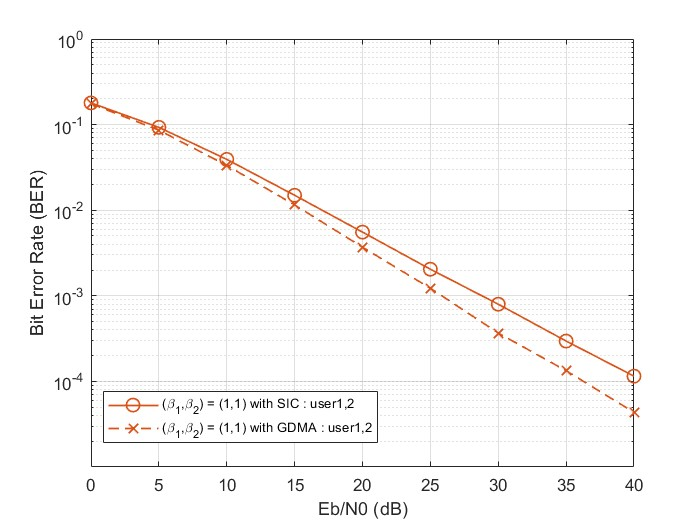
\includegraphics[width=0.9\linewidth]{figures/Chapter2/single_resource_beta1.jpg}}
    \caption{Users' BERs for single resource systems of $(\beta_1,\beta_2) = (1,1)$.}
    \label{fig:single-resource-ber-1-1}
\end{figure}
\begin{figure}[htbp]
    \centering
    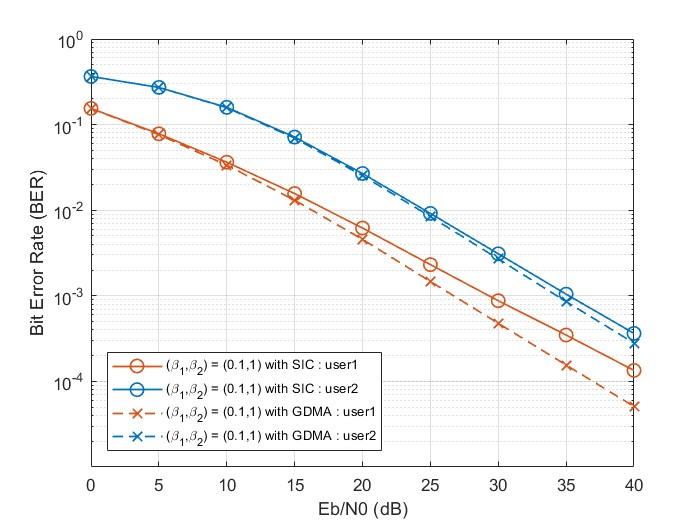
\includegraphics[width=0.9\linewidth]{figures/Chapter2/single_resource_beta0.1.jpg}
    \caption{Users' BERs for single resource systems of $(\beta_1,\beta_2) = (1,0.1)$.}
    \label{fig:single-resource-ber-1-0-1}
\end{figure}
\begin{figure}[htbp]
    \centering
    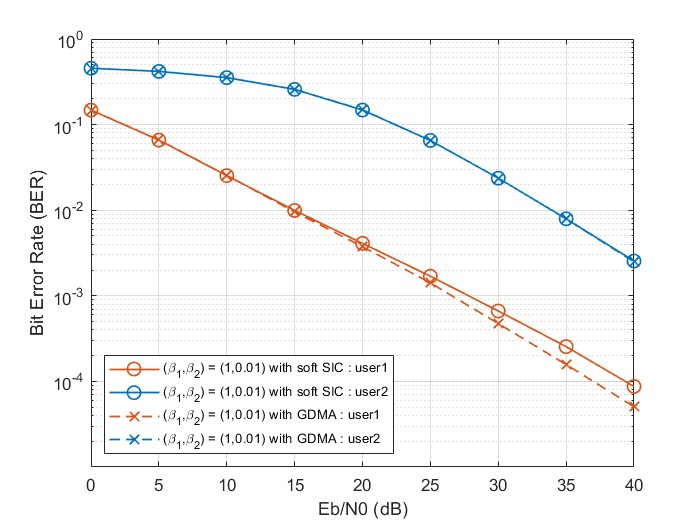
\includegraphics[width=0.9\linewidth]{figures/Chapter2/single_resource_beta0.01.jpg}
    \caption{Users' BERs for single resource systems of $(\beta_1,\beta_2) = (1,0.01)$.}
    \label{fig:single-resource-ber-1-0-01}
\end{figure}
\begin{figure}[htbp]
    \centering
    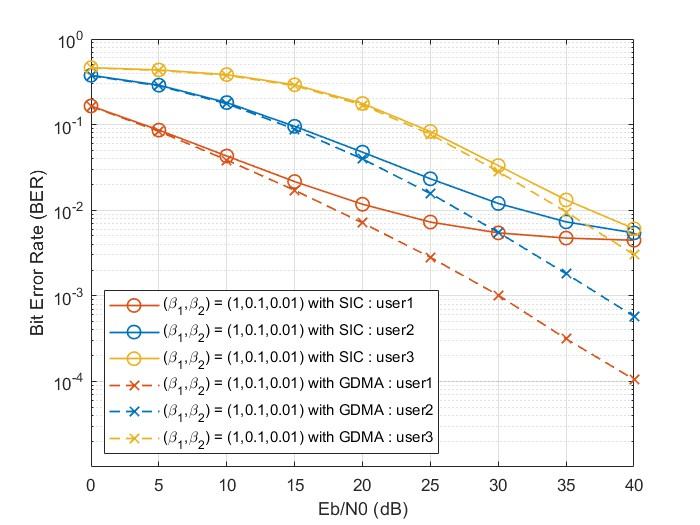
\includegraphics[width=0.9\linewidth]{figures/Chapter2/single_resource_beta0.1_U3.jpg}
    \caption{Users' BERs for single resource systems of $(\beta_1,\beta_2,\beta_3) = (1,0.1,0.01)$.}
    \label{fig:single-resource-ber-1-0-1-0-01}
\end{figure}





